% A Tour of Pollis AI+ — draft 1 (17 October 2026)
% The layout of The Pollis Guide: one topic per two-page spread, starting on an even (left-hand) page.
% Part one, The AI Ecosystem, explains the ideas behind Pollis AI+ to readers who have never met them
% at a technical level: language models in the cloud and on your computer, local model runners, coding
% agents and their harnesses, agent skills, MCP servers and orchestration, with examples from Pollis.
% Every statement about Pollis is checked against what it does today; what is not built yet is said to be
% not available.
% Compile with: latexmk -pdf pollis_ai_tour.tex
\documentclass[10pt,a4paper,twoside]{article}

\usepackage[a4paper,inner=18mm,outer=16mm,top=17mm,bottom=17mm,headsep=5mm,footskip=8mm]{geometry}
\usepackage[T1]{fontenc}
\usepackage[default,semibold]{sourcesanspro}
\usepackage{microtype}
\usepackage{graphicx}
\usepackage[table]{xcolor}
\usepackage{tikz}
\usetikzlibrary{arrows.meta,positioning,fit}
\usepackage[most]{tcolorbox}
\usepackage{fontawesome5}
\usepackage{tabularx}
\usepackage{enumitem}
\usepackage{fancyhdr}
\usepackage[hidelinks]{hyperref}

% ---------------------------------------------------------------- placeholders
\newcommand{\tourdate}{17 October 2026}
\newcommand{\downloadlink}{\href{https://github.com/saragga/pollis/releases/latest}{github.com/saragga/pollis/releases/latest}}
\newcommand{\contactemail}{\href{mailto:contact@pollis.org}{contact@pollis.org}}

% ---------------------------------------------------------------- colours (as in A Tour of Pollis)
\definecolor{navy}{HTML}{1C3A5E}
\definecolor{pblue}{HTML}{3B78B5}
\definecolor{amber}{HTML}{F2B33D}
\definecolor{deepamber}{HTML}{D9902A}
\definecolor{pale}{HTML}{EEF3F9}
\definecolor{ink}{HTML}{2A2F36}
\definecolor{soft}{HTML}{5E6773}
\definecolor{logonavy}{HTML}{173D63}
\definecolor{logodark}{HTML}{C98A1E}
\definecolor{logoamber}{HTML}{F2B446}
\definecolor{logocream}{HTML}{FEEFD2}
\color{ink}

% ---------------------------------------------------------------- layout
\setlength{\parindent}{0pt}
\setlength{\parskip}{3pt}
\setlist{nosep,leftmargin=*,itemsep=1.5pt}

% The topic's name in the head of both pages of its spread, page numbers on the outer edges
\newcommand{\topicname}{}
\pagestyle{fancy}
\fancyhf{}
\renewcommand{\headrulewidth}{0pt}
\fancyhead[LE,RO]{\footnotesize\color{soft}\topicname}
\fancyhead[RE,LO]{\footnotesize\color{soft}\textbf{A Tour of Pollis AI+}}
\fancyfoot[LE,RO]{\footnotesize\color{soft}\thepage}

% The Pollis logo, redrawn so it prints sharply at any size (as in A Tour of Pollis)
\newcommand{\pollislogo}[1]{%
  \begin{tikzpicture}[x=#1/512,y=-#1/512,baseline=(current bounding box.center)]
    \fill[logonavy] (0,0) rectangle (512,512);
    \fill[logodark] (36,422) -- (104,256) -- (172,422) -- cycle;
    \fill[logoamber] (104,422) -- (203,180) -- (302,422) -- cycle;
    \fill[logocream] (203,422) -- (339,89) -- (476,422) -- cycle;
  \end{tikzpicture}}

% A new topic: starts on the next even page, so its two pages face each other.
% #1 title, #2 where it is in Pollis, #3 what it is for, in one sentence.
\newcommand{\topic}[3]{%
  \clearpage
  \ifodd\value{page}\hbox{}\thispagestyle{empty}\clearpage\fi
  \renewcommand{\topicname}{#1}%
  {\color{navy}\fontsize{20}{24}\selectfont\bfseries #1}\par\vspace{2pt}
  {\color{deepamber}\small\bfseries #2}\par\vspace{3pt}
  {\color{soft}#3}\par\vspace{5pt}
  {\color{amber}\rule{\linewidth}{0.6pt}}\par\vspace{3pt}}

\newcommand{\subhead}[1]{\par\vspace{5pt}{\color{navy}\large\bfseries #1}\par\vspace{1pt}}
% A menu path or a button, as Pollis shows it
\newcommand{\ui}[1]{\textbf{#1}}
% A setting's id
\newcommand{\setting}[1]{\texttt{\small #1}}
% Something you type, or a command line
\newcommand{\cmd}[1]{\texttt{\small #1}}
% A request you could give an agent, in your own words
\newcommand{\ask}[1]{\par\vspace{1pt}{\color{pblue}\faComment[regular]}\enspace\emph{#1}\par}

% A plain box for limits and examples, and one for cautions
\newtcolorbox{note}[1]{enhanced, colback=pale, colframe=pale, boxrule=0pt, sharp corners,
  left=6pt, right=6pt, top=4pt, bottom=4pt, fontupper=\small,
  before upper={{\color{navy}\bfseries #1}\par\smallskip}}
\newtcolorbox{caution}[1]{enhanced, colback=white, colframe=amber, boxrule=0pt, leftrule=2.5pt,
  sharp corners, left=6pt, right=6pt, top=3pt, bottom=3pt, fontupper=\small,
  before upper={{\color{deepamber}\bfseries #1}\par\smallskip}}

% "See also": the related spreads
\newcommand{\seealso}[1]{\par\vspace{4pt}{\small\color{soft}\textbf{See also}\enspace #1}\par}

% A two-column table that fills the line: a term, and what it means
\newenvironment{pairs}[1][0.28]{\par\small\renewcommand{\arraystretch}{1.3}%
  \tabularx{\linewidth}{@{}>{\raggedright\arraybackslash\bfseries}p{#1\linewidth}>{\raggedright\arraybackslash}X@{}}}
  {\endtabularx\par}

% Boxes of the diagrams
\tikzset{
  box/.style={draw=navy, line width=0.6pt, fill=white, rounded corners=2pt, align=center,
    font=\small, inner sep=5pt, text width=#1},
  box/.default=26mm,
  hot/.style={box=#1, fill=pale},
  hot/.default=26mm,
  flow/.style={-{Stealth[length=5pt]}, line width=0.7pt, color=deepamber},
  both/.style={{Stealth[length=5pt]}-{Stealth[length=5pt]}, line width=0.7pt, color=deepamber},
  tag/.style={font=\scriptsize\itshape, color=soft, align=center},
}

\begin{document}

% =====================================================================
% PAGE 1 — COVER AND CONTENTS
% =====================================================================
\thispagestyle{empty}
\begin{minipage}[c]{24mm}\pollislogo{22mm}\end{minipage}%
\begin{minipage}[c]{0.8\linewidth}
  {\color{navy}\fontsize{36}{40}\selectfont\bfseries A Tour of Pollis AI+}\par\vspace{3pt}
  {\color{soft}\Large Pollis and AI, working together}
\end{minipage}

\vspace{12mm}
\begin{minipage}[t]{0.52\linewidth}\vspace{0pt}
\subhead{Pollis with or without AI}
AI is off by default, and Pollis works fully without it: every panel, notebook and workflow runs
without AI. Pollis AI+ is for those who want AI beside them: to write a new panel, a toolbox, a method
or its vignette, or to polish a report.

\subhead{Part one: The AI Ecosystem}
Talk about AI comes with many new words: language models, runners, agents, harnesses, skills, MCP
servers, orchestration. This part explains them for readers who have never met them at a technical
level: what each one is, how they fit together, and where each one is in Pollis, with examples.
Each topic takes two facing pages; read them in order the first time, since each builds on the one
before. Page 14 puts them all in one picture, with the words to know.

\smallskip
Menu paths are written \ui{Compose > Coding Agents}, and buttons as they appear, such as \ui{Use}.
What you could ask an agent is written
\ask{like this.}
This tour describes Pollis as it is on \tourdate. What is planned but not available yet is said to be
not available.

\subhead{Getting Pollis}
Pollis is free and open source, for Windows, macOS and Linux:\\ \downloadlink.\\
Questions and problems: \ui{Help > Report Issue}, or \contactemail.
\end{minipage}\hfill
\begin{minipage}[t]{0.40\linewidth}\vspace{0pt}
\begin{tcolorbox}[enhanced, colback=white, colframe=amber, boxrule=0pt, leftrule=2pt, sharp corners,
  left=8pt, right=0pt, top=2pt, bottom=2pt]
{\color{navy}\large\bfseries Contents}\par\medskip
{\color{soft}\small\bfseries The AI Ecosystem}\par\smallskip
\renewcommand{\arraystretch}{1.25}
\begin{tabular}{@{}r@{\enspace}l@{}}
{\color{deepamber}\bfseries 2} & Language Models\\
{\color{deepamber}\bfseries 4} & Local Model Runners\\
{\color{deepamber}\bfseries 6} & Coding Agents and Harnesses\\
{\color{deepamber}\bfseries 8} & Agent Skills\\
{\color{deepamber}\bfseries 10} & MCP Servers\\
{\color{deepamber}\bfseries 12} & Orchestration\\
{\color{deepamber}\bfseries 14} & The Whole Picture
\end{tabular}
\end{tcolorbox}
\end{minipage}

\vfill
{\color{soft}\small
\textcopyright\ 2026 Antonio Saragga Seabra\enspace·\enspace Licensed under \href{https://creativecommons.org/licenses/by-sa/4.0/}{CC BY-SA 4.0}\enspace·\enspace Draft, \tourdate}

% =====================================================================
% PAGES 2–3 — LANGUAGE MODELS
% =====================================================================
\topic{Language Models}{In the cloud · On your computer}{What a language model is, what it does well and badly, and the difference between one in the cloud and one on your computer.}

\subhead{What a language model is}
A \emph{large language model}, or \emph{LLM}, is a program trained on a vast amount of text to do one
thing: given some text, continue it. It writes one small piece at a time, a \emph{token}, which is a
word or part of a word, each one chosen to follow well from everything before it. Repeated thousands of
times, this gives answers, explanations, summaries and code. Claude, GPT and Gemini are language
models; so are Gemma, Llama, Qwen and Mistral.

\begin{note}{Example}
Ask a model \emph{``Write Julia code that fits a linear regression of y on x''} and it writes code,
because it has read a great deal of code like it. It has not run that code, and does not know whether it
works: it has written the most likely continuation of your request.
\end{note}

\subhead{What follows from how it works}
\begin{itemize}
  \item \textbf{It can be fluently wrong.} A confident answer is not a checked one. A model may call a
    function a Julia package does not have, or cite an article that was never published. This is why
    Pollis holds AI work to checks it does not write itself: the tests of a new method are the values
    the article publishes, and a new panel must pass Pollis' validator.
  \item \textbf{It knows the world up to a date}, its \emph{knowledge cutoff}. A package released after
    it, or a function renamed since, it does not know, unless it is told. Telling it is the job of
    skills (page 8) and MCP servers (page 10).
  \item \textbf{It reads a limited amount at once}, its \emph{context window}: your request, the files
    it was shown, the conversation so far. What is not in the window, it does not see. When the window
    fills up, the program around the model has to drop or summarise the earlier parts.
  \item \textbf{It does not remember you.} Each conversation starts afresh, unless the program around
    it keeps notes and shows them to the model next time.
  \item \textbf{Its answers vary.} The same request can give a different answer each time.
\end{itemize}

\subhead{A model alone cannot act}
A model only writes text. It cannot open your files, run Julia or look anything up. Everything beyond
writing text is done by a program around it: for a coding agent, its \emph{harness} (page 6).

\newpage
\subhead{Cloud models}
Most of the strongest models are run by companies in their data centres: Anthropic's Claude, OpenAI's
GPT, Google's Gemini and others. You reach them over the internet, with an account.
\begin{itemize}
  \item \textbf{Strong and fast}, with nothing to install but the program that talks to them.
  \item \textbf{They cost money}: a subscription, or a price per token read and written. A long task
    reads and writes many tokens. This is why every Pollis menu item that starts an agent carries a
    sparkle: it runs on your agent's account.
  \item \textbf{Your text goes to the provider}: your request, and every file the agent shows the
    model. What the provider may do with it is in its terms.
  \item \textbf{They need the internet.}
\end{itemize}

\subhead{Local models}
An \emph{open-weight} model is one whose trained numbers, its \emph{weights}, are published, so anyone
can download it and run it on their own computer: Google's Gemma, Meta's Llama, Alibaba's Qwen,
Mistral's models and OpenAI's gpt-oss are examples.
\begin{itemize}
  \item \textbf{Free}, once downloaded.
  \item \textbf{Private}: nothing you give it leaves your computer.
  \item \textbf{Offline}: it works on a train or a plane.
  \item \textbf{Smaller}, so weaker on hard tasks, and slower on a laptop than in a data centre. Your
    computer's memory limits which models it can run.
\end{itemize}

\begin{center}\small\renewcommand{\arraystretch}{1.3}
\begin{tabularx}{\linewidth}{@{}>{\bfseries}lXX@{}}
 & \textbf{Cloud model} & \textbf{Local model}\\\hline
Runs on & the provider's computers & yours\\
Costs & a subscription or a price per token & nothing, after the download\\
Your text & is sent to the provider & stays on your computer\\
Internet & needed & not needed\\
Best for & hard tasks, where a mistake costs most & small tasks, private data, no budget\\
\end{tabularx}
\end{center}

\begin{note}{In Pollis}
Some tasks are small: \ui{Polish with Agent} tidies the wording of a report. Others are hard:
\ui{Write a Method} must reproduce an article's tables to the digits printed. A small, fast or local
model suits the first; the second is where a strong model pays for itself. \ui{Model Routing} (page 12)
lets you make that choice once for each task.
\end{note}

\seealso{Local Model Runners, page 4.\quad Orchestration, page 12.}

% =====================================================================
% PAGES 4–5 — LOCAL MODEL RUNNERS
% =====================================================================
\topic{Local Model Runners}{Compose > Local Models > Local Model Runners}{The programs that run a language model on your own computer.}

\subhead{Why a runner is needed}
A downloaded model is a large file of numbers; on its own, it does nothing. A \emph{runner} is a program
that loads the file into memory, computes with it, on the processor or the graphics chip, and
\emph{serves} it: it waits at an address on your computer, so that other programs can send it text and
get the model's answer back, as they would from a cloud model. The model file is the recording; the
runner is the player.

\subhead{Addresses and APIs}
A runner serves its model at an address such as \cmd{http://localhost:11434}. \cmd{localhost} means
\emph{this computer}; \cmd{11434} is the \emph{port}, a door number, so that several programs can serve
at once. Programs talk to it through an \emph{API}, an agreed way of asking and answering. The APIs of
OpenAI and Anthropic have become common languages, and runners speak them. So a coding agent written for
a cloud model can be pointed at a local one by changing one address.

\subhead{The four runners Pollis knows}
\begin{center}\small\renewcommand{\arraystretch}{1.3}
\begin{tabularx}{\linewidth}{@{}>{\bfseries}lXl@{}}
\textbf{Runner} & \textbf{What it is} & \textbf{Port}\\\hline
Ollama & A program that downloads and runs models with one command; OpenAI and Anthropic APIs & 11434\\
LM Studio & A desktop app with a model browser; OpenAI and Anthropic APIs; runs MLX models on Apple silicon & 1234\\
llama.cpp & Its \cmd{llama-server}; OpenAI and Anthropic APIs & 8080\\
Apple MLX & Apple's framework for Macs with Apple silicon; its \cmd{mlx\_lm.server} speaks the OpenAI API & 8080\\
\end{tabularx}
\end{center}
\ui{Compose > Local Models > Local Model Runners} shows which runners are installed, with
\ui{Install Runner} for the others, and how each coding agent reaches each runner. Apple MLX is listed
only on a Mac.

\newpage
\subhead{Getting a model}
\ui{Hugging Face Models} and \ui{Kaggle Models}, the other entries of \ui{Compose > Local Models}, find
models to download. A runner can also fetch them itself. With Ollama, for example:
\begin{itemize}
  \item \cmd{ollama pull gemma3} downloads Google's Gemma 3;
  \item \cmd{ollama run gemma3} starts a chat with it in the terminal.
\end{itemize}

\subhead{Which size?}
A model's size is its number of weights, written in billions: a ``7B'' model has about seven billion.
Bigger is usually better, and needs more memory. A \emph{quantised} model keeps each weight in fewer
bits: a smaller file, slightly less accurate. The rule of thumb: the model's file must fit in your
computer's memory, with room to spare for the conversation.

\subhead{Example: a coding agent on a local model}
\begin{enumerate}[label=\arabic*.]
  \item Install Ollama: \ui{Install Runner}, on the Local Model Runners page.
  \item In \ui{Compose > Coding Agents}, under \ui{Local and Cloud Models}, use your agent's local
    command, such as \cmd{ollama launch claude -{}- \{prompt\}} for Claude Code, or
    \cmd{codex -{}-oss \{prompt\}} for Codex.
  \item Start a task, such as \ui{Compose > New Panels and Toolboxes > Create a Panel...}. The agent
    works exactly as before; only the model that answers it is now on your computer.
\end{enumerate}

\begin{note}{The agent is always local; the model may not be}
A coding agent always runs on your computer, in a terminal. What is \emph{local} or \emph{cloud} is the
model it talks to. ``A local agent'' usually means an agent on a local model.
\end{note}

\begin{caution}{Smaller models, simpler tasks}
A local model follows long instructions less reliably than a strong cloud model. Give it the light
tasks, and check what it produces, as you would any agent's work.
\end{caution}

\seealso{Language Models, page 2.\quad Coding Agents and Harnesses, page 6.}

% =====================================================================
% PAGES 6–7 — CODING AGENTS AND HARNESSES
% =====================================================================
\topic{Coding Agents and Harnesses}{Compose > Coding Agents}{A model that can act: what a coding agent is, and the harness that makes it one.}

\subhead{From a chat to an agent}
In a chat, you ask, the model answers with code, you copy it into Julia, run it, and paste the error
back. A \emph{coding agent} does the copying and the running itself: it reads your files, writes
changes, runs commands such as \cmd{julia}, reads what they print, and tries again, until the task is
done or it needs you.

\subhead{The harness}
The model is the agent's mind; the \emph{harness} is everything around it: a program on your computer,
in a terminal, that turns the model's text into actions.
\begin{itemize}
  \item \textbf{The loop.} It sends your request to the model, carries out what the model asks for,
    sends back the result, and repeats.
  \item \textbf{The tools.} Read a file, edit a file, search, run a command, fetch a web page. The model
    only asks; the harness does it.
  \item \textbf{The permissions.} Which actions need your yes first, such as running a command or
    writing outside the project folder.
  \item \textbf{The context.} What goes into the model's window at each step: its instructions, your
    files, the steps so far, summarised when the window fills up.
  \item \textbf{The memory.} Notes and project instructions kept in files between sessions.
\end{itemize}

\begin{center}
\begin{tikzpicture}[node distance=7mm and 9mm]
  \node[box=20mm] (you) {\textbf{You}\\{\scriptsize a request}};
  \node[hot=36mm, right=of you] (harness) {\textbf{The harness}\\{\scriptsize loop · tools · permissions\\context · memory}};
  \node[box=24mm, right=of harness] (model) {\textbf{The model}\\{\scriptsize cloud or local}};
  \node[box=40mm, below=of harness] (world) {\textbf{Your computer}\\{\scriptsize files · terminal · \cmd{julia} · the web}};
  \draw[both] (you) -- (harness);
  \draw[both] (harness) -- node[tag, above] {text} (model);
  \draw[both] (harness) -- node[tag, right] {actions, results} (world);
  \node[draw=deepamber, dashed, rounded corners=3pt, inner sep=4pt, fit=(harness) (model),
    label={[tag]above:a coding agent = model + harness}] {};
\end{tikzpicture}
\end{center}

\newpage
\subhead{The agents Pollis knows}
\ui{Compose > Coding Agents} lists three agents, each with the command that starts it, and
another that starts it on a local model. Same harness, different model.
\begin{center}\small\renewcommand{\arraystretch}{1.3}
\begin{tabularx}{\linewidth}{@{}>{\bfseries}lXX@{}}
\textbf{Agent} & \textbf{Command} & \textbf{On a local model}\\\hline
Claude Code & \cmd{claude \{prompt\}} & \cmd{ollama launch claude -{}- \{prompt\}}\\
Codex & \cmd{codex \{prompt\}} & \cmd{codex -{}-oss \{prompt\}}\\
OpenCode & \cmd{opencode -{}-prompt \{prompt\}} & \cmd{ollama launch opencode -{}- -{}-prompt \{prompt\}}\\
\end{tabularx}
\end{center}
\cmd{\{prompt\}} is where Pollis puts the first message. Click \ui{Use} beside yours; for any other agent,
type its command line under \ui{Other Agent}.

\subhead{Example: Create a Panel, step by step}
\begin{enumerate}[label=\arabic*.]
  \item Choose \ui{Compose > New Panels and Toolboxes > Create a Panel...}. Pollis opens a terminal and
    starts your agent with a first message: \emph{``Read the skill \ldots\ and follow its instructions
    to create a new Pollis panel with me.''}
  \item The agent reads the skill (page 8) and asks you, in one message, what the panel is for, the
    methods it covers and the Julia packages to use. It proposes a plan and waits for your yes.
  \item It writes the panel's TOML file, its wiki pages and its notebook tutorials.
  \item It runs Pollis' validator on them, reads the errors, fixes them, and runs it again until it
    passes.
  \item It packages the panel as a toolbox, ready to install or share.
\end{enumerate}
Steps 3 and 4 are the loop: write, check, read the result, correct. A chat cannot do this; an agent can,
because its harness can run the validator.

\begin{caution}{An agent works on your files}
It reads and writes files, and runs commands. Read what it proposes before you say yes, and check its
results, as you would a colleague's.
\end{caution}

\seealso{Agent Skills, page 8.\quad Orchestration, page 12.}

% =====================================================================
% PAGES 8–9 — AGENT SKILLS
% =====================================================================
\topic{Agent Skills}{Compose > Agent Skills}{Know-how written down, so that an agent can do a task it was never trained for.}

\subhead{Why an agent needs skills}
A model knows a great deal in general, and nothing about Pollis' panel format, its registry rules or how
its vignettes look: they are too recent, or were never in its training text. Without help, it would
guess. A \emph{skill} is the help: the know-how for one task, written down for the agent to read.

\subhead{What a skill is}
A folder with a file named \cmd{SKILL.md}: a name, a short description of when to use it, and the
instructions. Beside it there can be reference pages and scripts. It is plain text: anyone can read it,
and change it, with no retraining of any model. Think of a laboratory protocol: the same protocol makes
a new member of the team do the procedure the way the team does it.

\subhead{How an agent uses one}
An agent first reads only the names and descriptions of its skills, which is cheap. When a request
matches one, such as
\ask{Build a toolbox for my course from these panels.}
it reads that skill in full, then follows it. Pollis' agent tasks go straight to the point: their first
message names the skill to read.

\subhead{Scripts that check}
The best skills do not only say \emph{check your work}; they bring a program that checks it. The
create-panel skill comes with \cmd{validatePanel.mjs}, Pollis' validator; the write-method skill runs the
method's tests against the published values. Instructions say what to do; the checks show whether it was
done.

\newpage
\subhead{The Pollis skills}
\begin{pairs}[0.2]
create-panel & Write a new panel on a topic you choose: its TOML file, wiki pages and notebook
  tutorials; check it with the validator; package it as a toolbox.\\
package-toolbox & Build a toolbox from the menu entries you pick, in the menus and order you want: for
  example, one toolbox per course.\\
write-method & Write the Julia code of a published method, so that it reproduces the article's tables to
  the digits printed, tested with Pollis' package script.\\
prepare-method & Bring a method up to the rules of the Pollis registry, such as a docstring for every
  exported name, without changing what it computes.\\
write-vignette & Write a method's vignette: a two-page document that sets its results beside the
  published ones.\\
references & Cite as Author (year), with all authors written out, each linked to its entry in the
  references, from the Pollis library, with its DOI.\\
\end{pairs}

\subhead{Examples}
\ask{Write a method from this article: these are its tables.}
The write-method skill turns every published value into a test before any code is written, then has the
agent write the code until the tests pass.
\ask{Add the references to this report.}
The references skill makes the agent cite from the Pollis library, never from memory, so that no
reference is invented.

\subhead{In Pollis}
\ui{Compose > Agent Skills} lists the skills, downloaded in their latest version when the page opens,
each with its \ui{Tasks} and \ui{Example Requests}. \ui{View Skill} opens one; \ui{Run with My Agent}
starts your agent on it. \ui{Install Skills}, on the \ui{Compose > Coding Agents} page, installs them
for your agent, so that it knows them in any folder, even outside Pollis.

\begin{note}{Skills and MCP servers}
A skill gives an agent \emph{know-how}: how to do a task. An MCP server, on the next spread, gives it
\emph{reach}: data and services it could not get to before.
\end{note}

\seealso{Coding Agents and Harnesses, page 6.\quad MCP Servers, page 10.}

% =====================================================================
% PAGES 10–11 — MCP SERVERS
% =====================================================================
\topic{MCP Servers}{Compose > MCP Servers · Extensions pane > MCP Servers - Recommended}{New tools for an agent: data and services it can reach, in a form every agent understands.}

\subhead{What MCP is}
A harness comes with general tools: read files, run commands. An \emph{MCP server} adds tools of a
particular service: search FRED's series, query a database, read your Zotero library. MCP, the
\emph{Model Context Protocol}, is the agreed way an agent and a server talk, so that one server works
with every agent that speaks it. Think of a USB plug: the same plug fits every computer.

\subhead{How a tool is used}
Each server lists its tools, with a description of each. The model reads the descriptions and, when one
fits your request, asks for it; the harness calls the server, and the answer goes into the model's
context window, where the model can use it.

\subhead{Remote and local servers}
A \emph{remote} server runs at its provider, at a web address: FRED and Hugging Face. A \emph{local}
server is a program on your computer that the agent starts when it needs it: DuckDB, arXiv and Zotero,
run with \cmd{uvx}, part of the uv program, which fetches what they need.

\subhead{The five servers Pollis recommends}
\begin{center}\small\renewcommand{\arraystretch}{1.3}
\begin{tabularx}{\linewidth}{@{}>{\bfseries}lXl@{}}
\textbf{Server} & \textbf{What it gives an agent} & \textbf{Runs}\\\hline
FRED & Economic time series from the Federal Reserve Bank of St.\ Louis: search, notes, observations & remote\\
Hugging Face & The Hub's models, datasets and Spaces: search, details, files & remote\\
DuckDB & SQL on CSV, Parquet and JSON files, in an in-memory database & local\\
arXiv & Papers on arXiv: search, download, read & local\\
Zotero & Your Zotero library, read only: references, BibTeX, full text & local\\
\end{tabularx}
\end{center}

\newpage
\subhead{Examples}
\ask{Fetch the monthly US unemployment rate, UNRATE, since 2000, and save it as a CSV file.}
FRED finds the series and its observations; the agent writes the file.
\ask{Which datasets on Hugging Face have daily stock returns?}
\ask{Load sales.csv and give me the average sale by region.}
DuckDB runs the SQL query on the file, on your computer.
\ask{Find recent papers on conformal prediction for time series, and summarise their methods.}
\ask{Give me the BibTeX of Bollerslev (1986) from my Zotero library.}

\subhead{Setting one up}
\ui{Compose > MCP Servers} shows each server's tools, what it requires and its command, with an
\ui{Add} button for each coding agent (\ui{Add and Sign In} for FRED, which asks you to sign in). The
\ui{MCP Servers - Recommended} section of the Extensions pane lists the same servers; \ui{Set Up} opens
the page at that server.

\subhead{What leaves your computer}
\begin{center}\small\renewcommand{\arraystretch}{1.3}
\begin{tabularx}{\linewidth}{@{}>{\bfseries}lX@{}}
Remote server & Your request to it goes to its provider: your FRED searches go to the St.\ Louis Fed.\\
Local server & Its work stays on your computer; arXiv still downloads papers from arXiv.\\
Cloud model & Whatever a tool returns goes into the context, so it is sent to the model's provider: the
  full text of a Zotero reference, the rows of a DuckDB query.\\
Local model & With local servers too, nothing leaves your computer but what they fetch.\\
\end{tabularx}
\end{center}

\begin{caution}{Add only servers you trust}
A server is a program that acts for your agent: DuckDB can read and write files on your computer. And
text an agent fetches, a web page or a paper, may contain instructions written to mislead it. Prefer
well-known servers, and read what the agent proposes to do with what it fetched.
\end{caution}

\seealso{Agent Skills, page 8.\quad Orchestration, page 12.}

% =====================================================================
% PAGES 12–13 — ORCHESTRATION
% =====================================================================
\topic{Orchestration}{Compose > Orchestration}{Several models, or several agents, each doing the part it does best.}

\subhead{What orchestration is}
So far, one agent has done one task. \emph{Orchestration} arranges several: a cheap model for the small
tasks and a strong one for the hard, or two agents that check each other. As a conductor does not play,
but decides who plays when, orchestration writes no code; it decides which model or agent does what.

\subhead{The simplest kind: Model Routing}
Not every task needs the strongest model. \ui{Compose > Orchestration > Model Routing} has three
\emph{tiers}:
\begin{itemize}
  \item \ui{Light}: small tasks, on a fast, cheap or local model.
  \item \ui{Standard}: everyday tasks.
  \item \ui{Strong}: hard tasks, where a mistake costs most.
\end{itemize}
Each tier is the command line of an agent, with \cmd{\{prompt\}}. For example:
\begin{center}\small\renewcommand{\arraystretch}{1.3}
\begin{tabular}{@{}>{\bfseries}ll@{}}
Light & \cmd{ollama launch claude -{}- \{prompt\}}, on a local model, free\\
Standard & \cmd{claude -{}-model sonnet \{prompt\}}\\
Strong & \cmd{claude -{}-model opus \{prompt\}}\\
\end{tabular}
\end{center}
An empty tier runs your main agent, the one chosen in \ui{Compose > Coding Agents}, and so does a tier
whose program is not installed. Each task has a tier by default; in \ui{Tasks}, choose another.

\newpage
\begin{center}\small\renewcommand{\arraystretch}{1.3}
\begin{tabularx}{\linewidth}{@{}Xll@{}}
\textbf{Task} & \textbf{Menu} & \textbf{Tier}\\\hline
Polish with Agent & Reports & Light\\
Write a Vignette, Prepare for Registration & Methods & Standard\\
Package a Toolbox & New Panels and Toolboxes & Standard\\
Tables from the Article, Write a Method & Methods & Strong\\
Create a Panel, Create Panels from a Request & New Panels and Toolboxes & Strong\\
\end{tabularx}
\end{center}

\subhead{Why route?}
\begin{itemize}
  \item \textbf{Cost}: a small model costs a fraction of a strong one, and a local one nothing.
  \item \textbf{Speed}: small models answer sooner.
  \item \textbf{Privacy}: a local Light tier keeps its tasks on your computer.
  \item \textbf{Quality where it counts}: the tasks whose results must match published values get the
    strongest model.
\end{itemize}

\subhead{Agents that check each other}
A model's mistakes are not random: run the same model twice and it may make the same mistake twice. Two
\emph{different} models, or one model and a published value, do not share their blind spots. This is the
idea behind double data entry, where two people type the same form and every difference is looked at.
Three patterns in \ui{Compose > Orchestration} are built on it:
\begin{pairs}[0.36]
Writer and Checker... & one agent writes; another checks the work.\\
Two Independent Transcriptions... & two agents copy the same tables from an article, each on its own;
  where they differ, you decide.\\
Race... & several agents do the same task, and you compare what they produce.\\
\end{pairs}

\begin{note}{Not available yet}
\ui{Writer and Checker...}, \ui{Two Independent Transcriptions...} and \ui{Race...} are in the
\ui{Orchestration} menu but not built yet. Today, Pollis' checks are the tests from published values and
the panel validator.
\end{note}

\seealso{Language Models, page 2.\quad Coding Agents and Harnesses, page 6.}

% =====================================================================
% PAGES 14–15 — THE WHOLE PICTURE
% =====================================================================
\topic{The Whole Picture}{Compose}{How the pieces fit together, and the words to know.}

\begin{center}
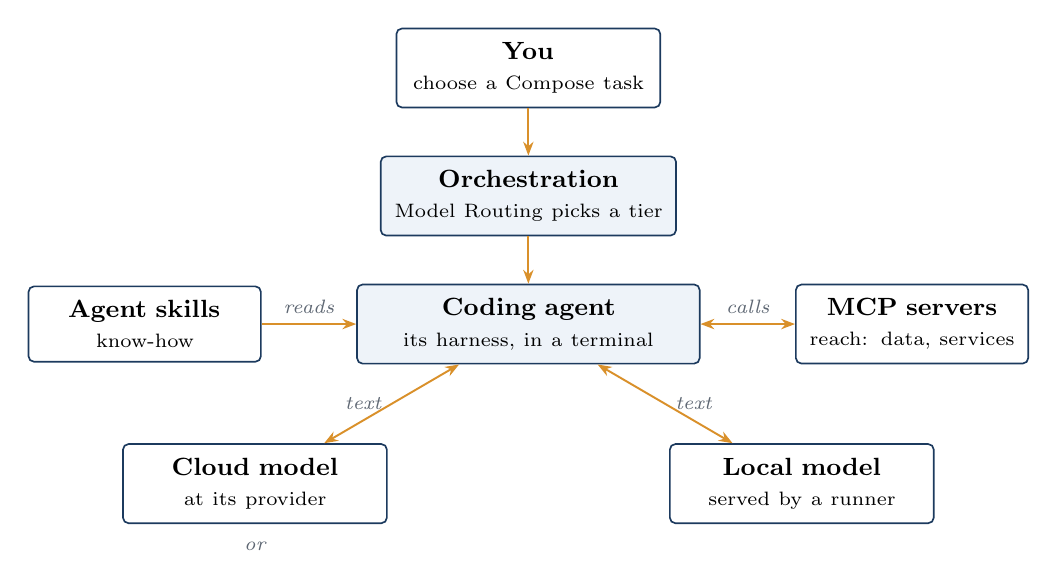
\begin{tikzpicture}[node distance=6mm and 7mm]
  \node[box=30mm] (you) {\textbf{You}\\{\scriptsize choose a Compose task}};
  \node[hot=34mm, below=of you] (route) {\textbf{Orchestration}\\{\scriptsize Model Routing picks a tier}};
  \node[hot=40mm, below=of route] (agent) {\textbf{Coding agent}\\{\scriptsize its harness, in a terminal}};
  \node[box=26mm, left=12mm of agent] (skills) {\textbf{Agent skills}\\{\scriptsize know-how}};
  \node[box=26mm, right=12mm of agent] (mcp) {\textbf{MCP servers}\\{\scriptsize reach: data, services}};
  \node[box=30mm, below left=10mm and -4mm of agent] (cloud) {\textbf{Cloud model}\\{\scriptsize at its provider}};
  \node[box=30mm, below right=10mm and -4mm of agent] (local) {\textbf{Local model}\\{\scriptsize served by a runner}};
  \draw[flow] (you) -- (route);
  \draw[flow] (route) -- (agent);
  \draw[flow] (skills) -- node[tag, above] {reads} (agent);
  \draw[both] (agent) -- node[tag, above] {calls} (mcp);
  \draw[both] (agent) -- node[tag, left] {text} (cloud);
  \draw[both] (agent) -- node[tag, right] {text} (local);
  \node[tag, below=1mm of cloud] {or};
\end{tikzpicture}
\end{center}

\subhead{One task, from start to finish}
You choose \ui{Compose > Under Construction...} and click \ui{Write Method} beside your method.
Model Routing sends the task to the \ui{Strong} tier. Pollis opens a terminal and starts that tier's
agent, with a first message naming the write-method skill and the method's test command. The agent
reads the skill; if the article is on arXiv, the arXiv server can fetch it; its model writes the code; its harness runs the tests
against the published values; and the loop goes on until every test passes. You read the numbers,
beside the published ones.

\newpage
\subhead{Words to know}
\begin{pairs}[0.24]
Language model (LLM) & A program that continues text, one token at a time; page 2.\\
Token & A word or part of a word: what models read and write, and what cloud models charge for.\\
Context window & What a model can read at once: the request, files, the conversation so far.\\
Knowledge cutoff & The date after which a model knows nothing, unless it is told.\\
Cloud model & A model run by its provider, reached over the internet with an account.\\
Open-weight model & A model whose weights are published, so it can run on your computer.\\
Local model & A model running on your computer: free, private, offline, smaller.\\
Weights & The trained numbers of a model; their count, in billions, is its size.\\
Quantised & Kept with fewer bits per weight: a smaller file, slightly less accurate.\\
Runner & A program that loads a model and serves it on your computer; page 4.\\
API & The agreed way programs ask and answer; runners speak the APIs of OpenAI and Anthropic.\\
Coding agent & A model that can act: it reads and writes files and runs commands; page 6.\\
Harness & The program around the model: loop, tools, permissions, context, memory.\\
Agent skill & Written know-how for one task, which the agent reads when it needs it; page 8.\\
MCP server & A server of tools an agent can use, through the Model Context Protocol; page 10.\\
Orchestration & Arranging several models or agents, each on the part it does best; page 12.\\
Tier & In Model Routing, Light, Standard or Strong: the agent a kind of task runs on.\\
\end{pairs}

\end{document}
